
% talvez remover esse slide
\begin{frame}{Cenário de execução}
    \begin{figure}
        \centering
        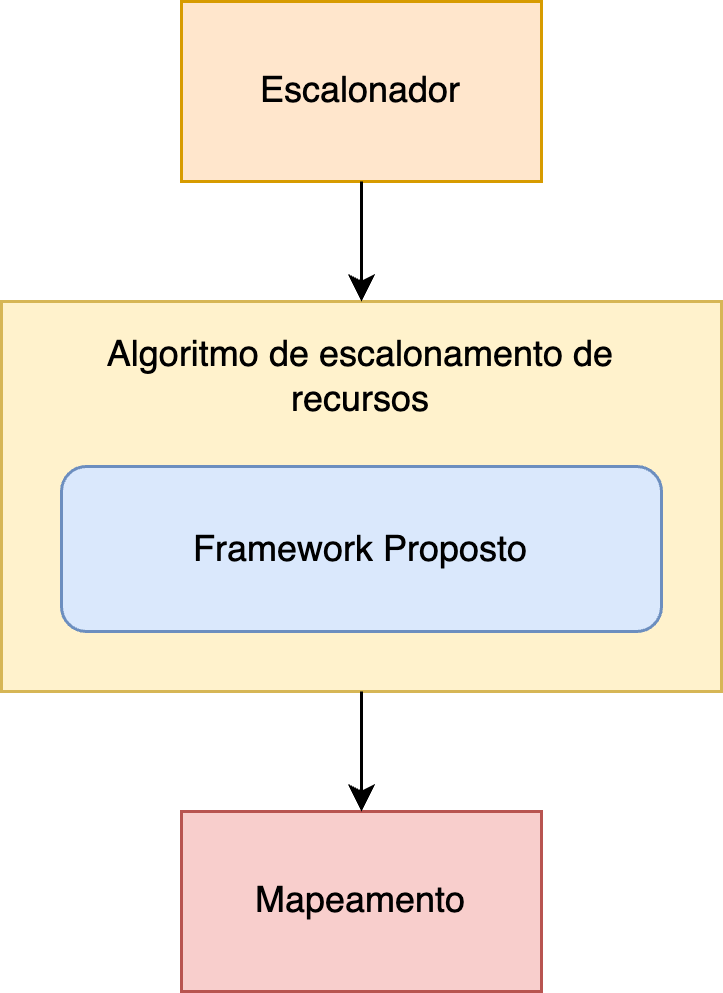
\includegraphics[width=0.5\textwidth]{Figuras/framework_usage.png}
    \end{figure}
\end{frame}

\begin{frame}{Código Exemplo}
    \begin{figure}
        \centering
        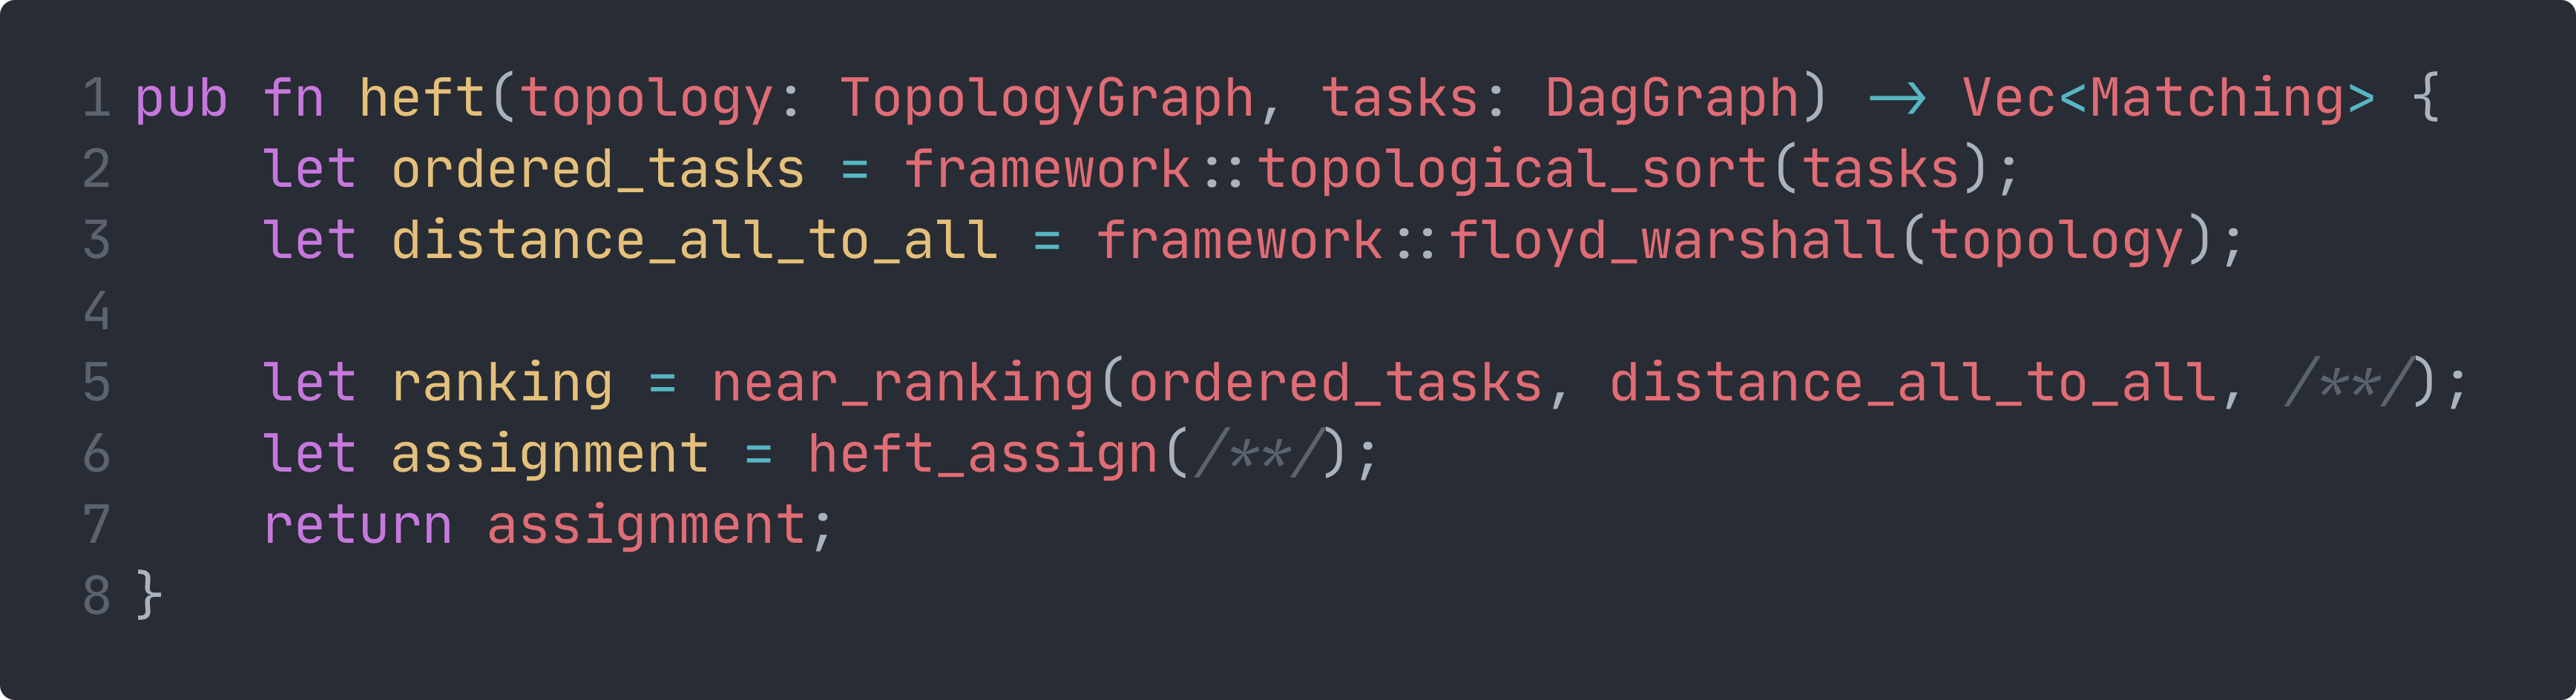
\includegraphics[width=\textwidth]{Figuras/code.png}
    \end{figure}
\end{frame}

\begin{frame}{Técnicas e Ferramentas}
    \begin{columns}
    \begin{column}{0.9\textwidth}
    Rust:
    \begin{itemize}
        \item[--] Linguagem moderna.
        \item[--] Segurança de memória.
        \item[--] Alto desempenho. 
        \item[--] \textit{Petgraph}.
        \item[--] \textit{Fearless Concurrency}.
        \item[--] \textit{Rayon}.
    \end{itemize}
    \end{column}

    \begin{column}{0.1\textwidth}
        \begin{figure}
            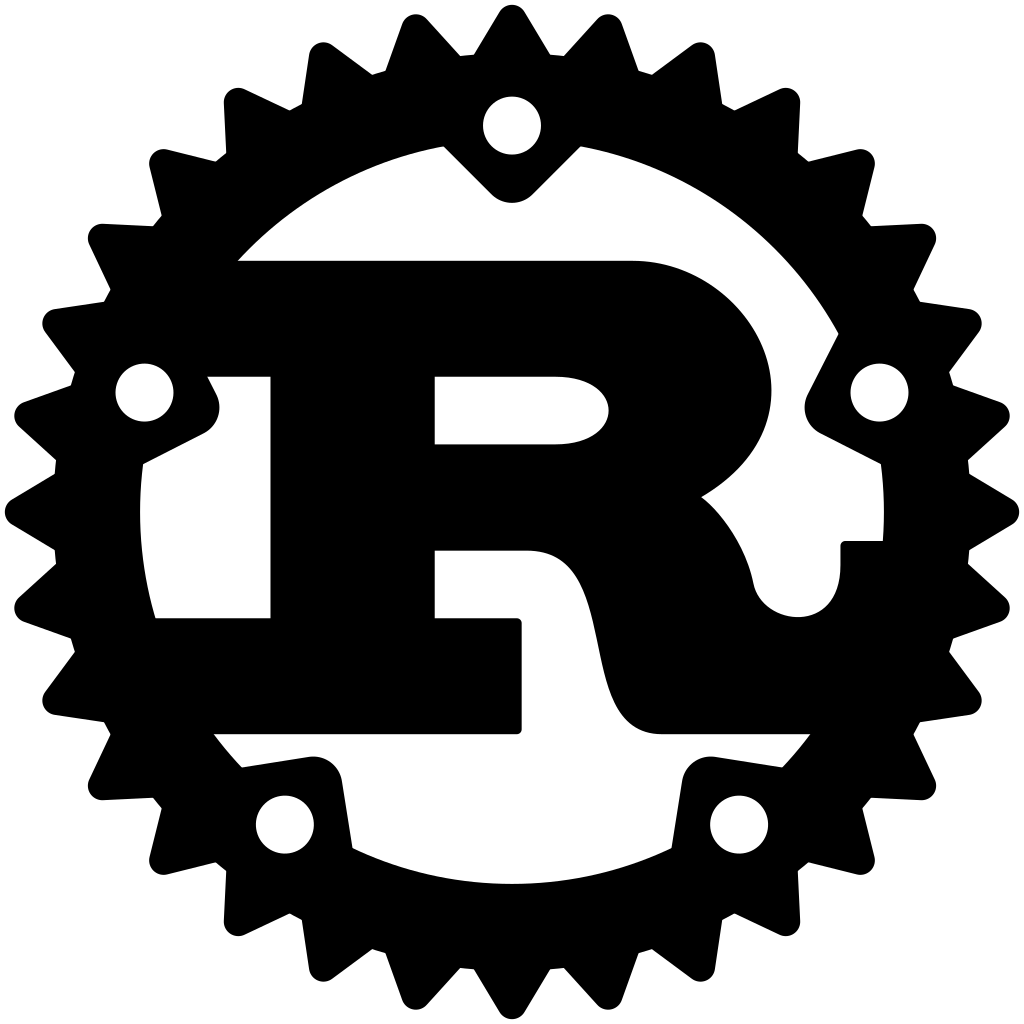
\includegraphics[width=\textwidth]{Figuras/Rust Logo.svg.png}
        \end{figure}
    \end{column}
    \end{columns}
\end{frame}

\begin{frame}{Fearless Concurrency}
    \begin{figure}
        \centering
        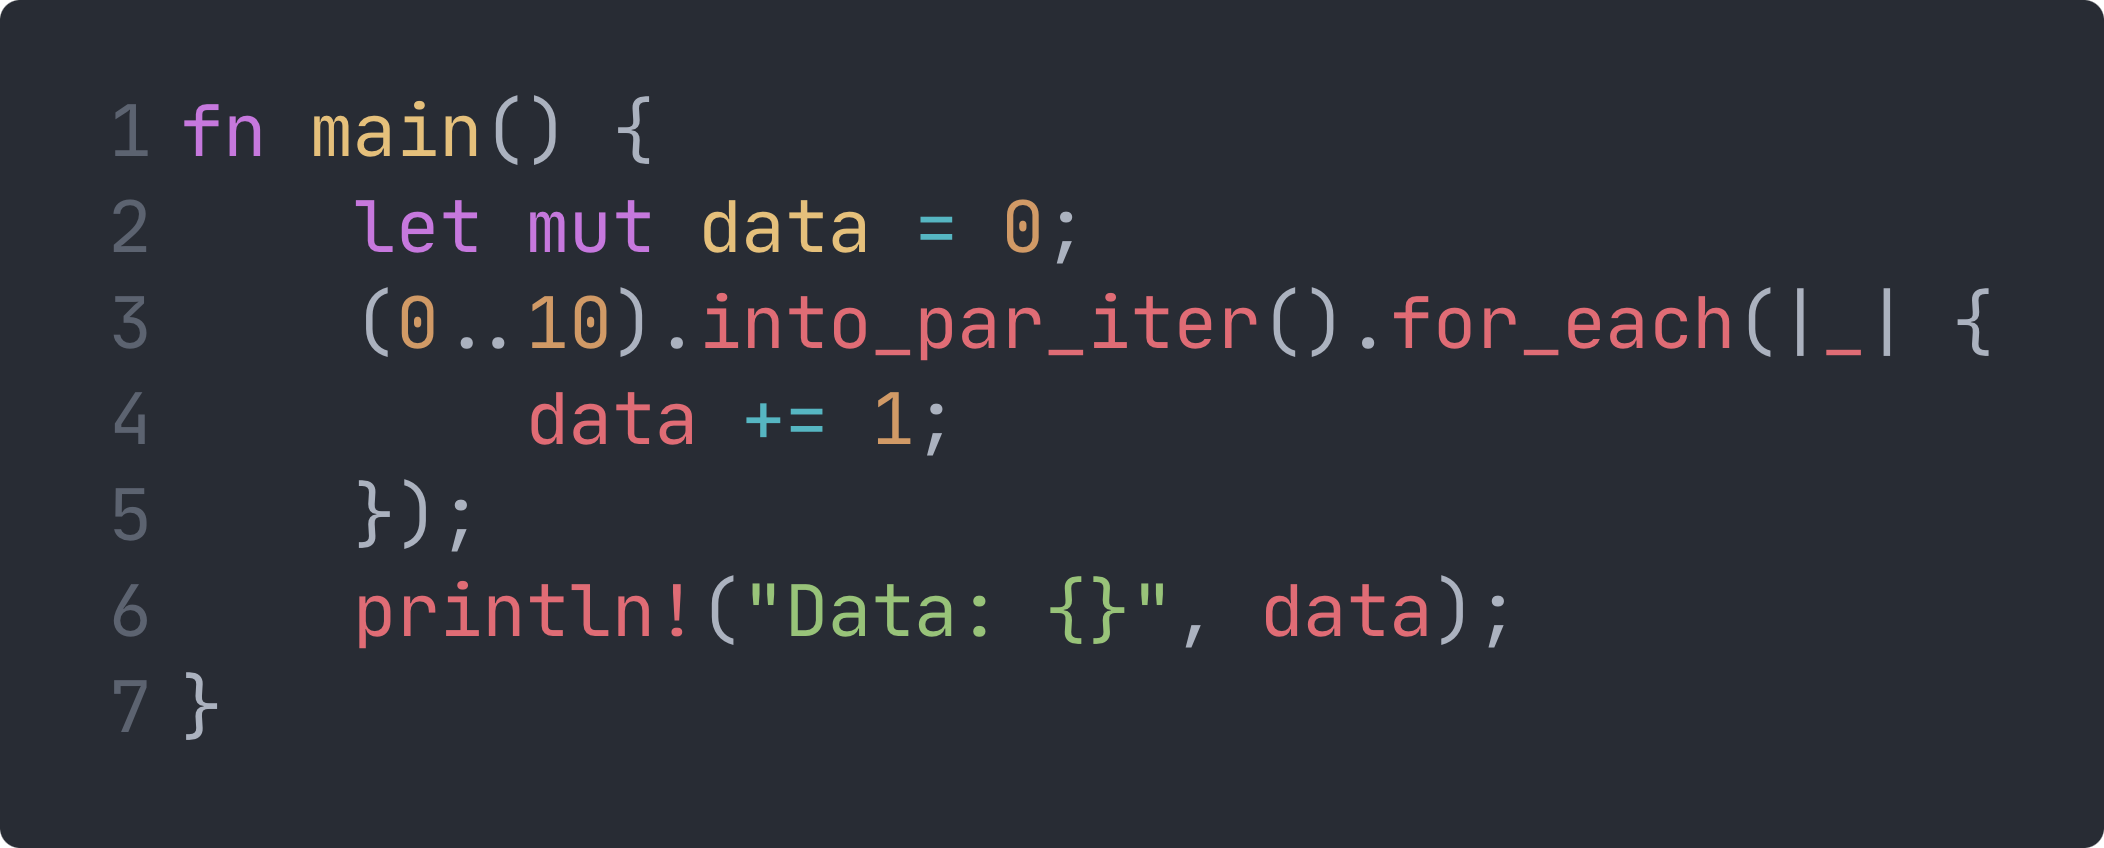
\includegraphics[width=\textwidth]{Figuras/fearlessconcurrency.png}
    \end{figure}
\end{frame}

\begin{frame}{Técnicas e Ferramentas}
    \begin{columns}
    \begin{column}{0.9\textwidth}
    C++:
    \begin{itemize}
        \item[--] Excelente suporte a \textit{GPUs}.
        \item[--] \textit{OpenAcc}.
        \item[--] Comunicação por meio de \textit{Foreign Function Interface}.
    \end{itemize}
    \end{column}

    \begin{column}{0.1\textwidth}
        \begin{figure}
            
\includegraphics[width=\textwidth]{Figuras/C++ Logo.png}
        \end{figure}
    \end{column}
    \end{columns}
\end{frame}

\begin{frame}{Cenário experimental}
    Métricas:
    \begin{itemize}
        \item[--] Speedup, Eficiência, Escalabilidade, Overhead, Utilização de recursos.
    \end{itemize}

    Base de dados aberta:
    \begin{itemize}
        \item[--] \textit{Politecnico di Milano}.
        \item[--] Dados reais e sintéticos.
        \item[--] Grafos de diversos tamanhos e formatos.
    \end{itemize}

    Infraestrutura local do LabP2D:
    \begin{itemize}
        \item[--] 2 CPUs Intel Xeon Silver 2.2GHz.
        \item[--] NVIDIA RTX 3090 24GB.
    \end{itemize}
\end{frame}
